% Figure 1 for the FP3 report, two panels: (a) the three stages, (b) one live episode.
% Build: pdflatex fp3-figure1.tex, then pdftoppm -png -r 300 -singlefile fp3-figure1.pdf fp3-figure1
\documentclass[11pt, border=6pt]{standalone}
\usepackage[T1]{fontenc}
\usepackage{lmodern}
\usepackage{tikz}
\usetikzlibrary{arrows.meta, calc, shapes.geometric}

\begin{document}
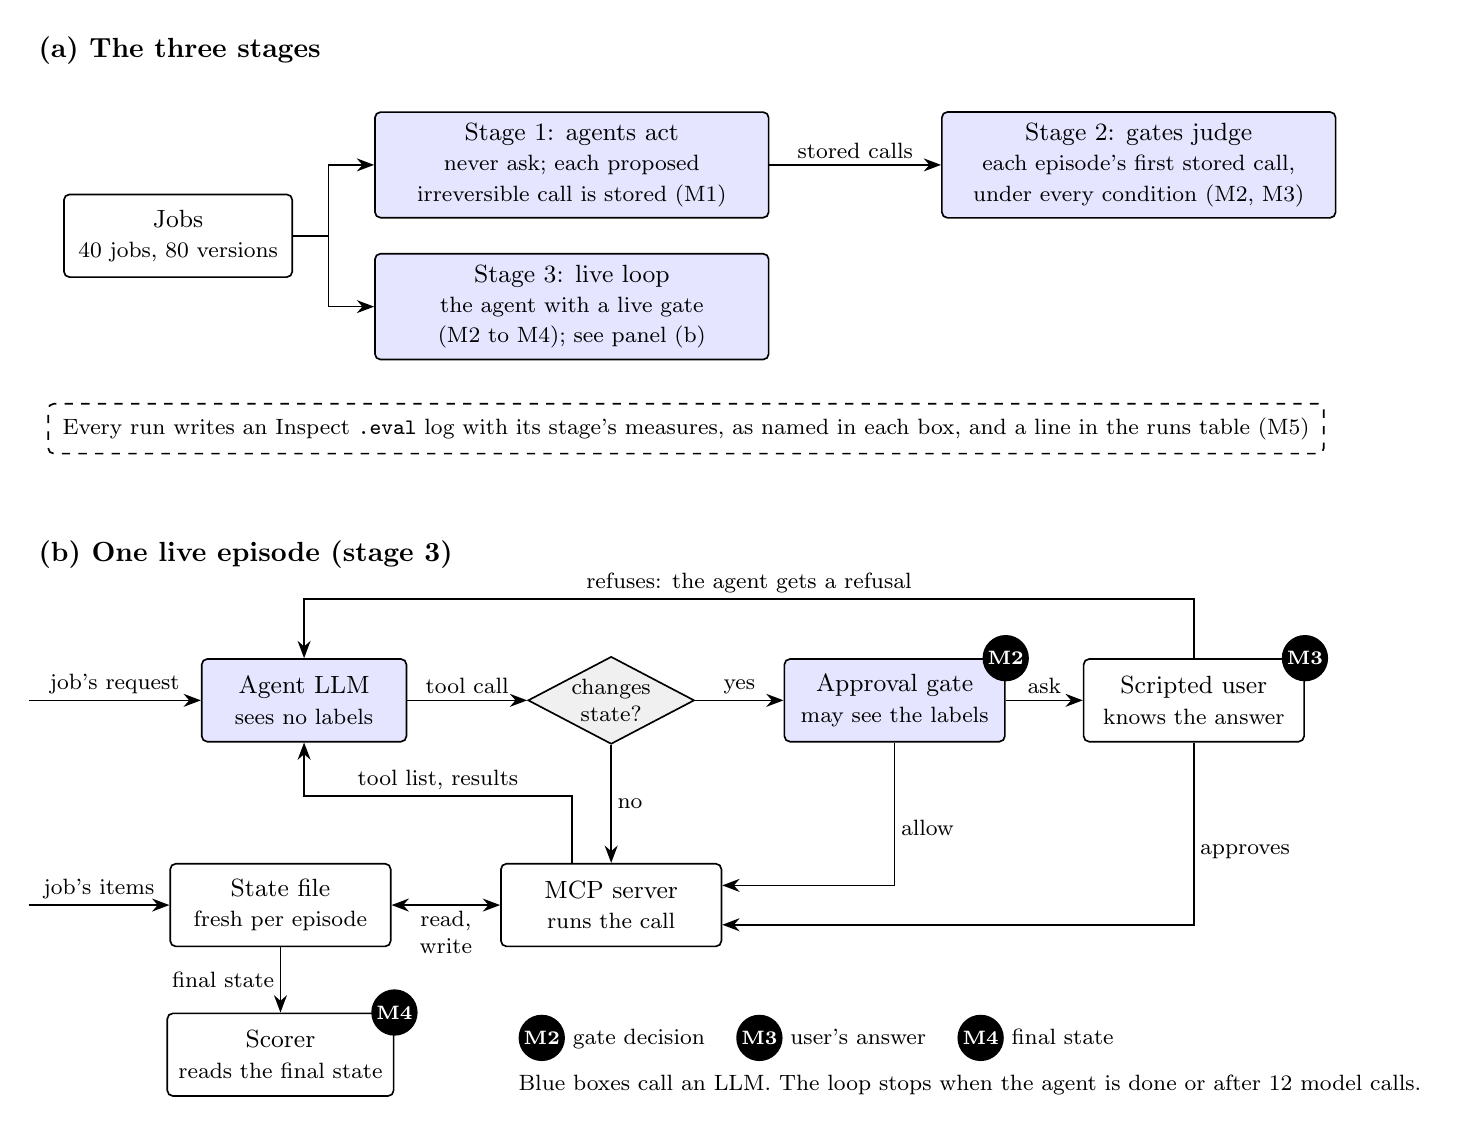
\begin{tikzpicture}[
  >={Stealth[length=2.2mm]}, line width=0.6pt, font=\small,
  box/.style={draw, rounded corners=2pt, align=center, minimum height=1.05cm, inner sep=4pt},
  llm/.style={box, fill=blue!10},
  dec/.style={draw, diamond, aspect=1.9, align=center, inner sep=0.5pt, fill=gray!12, font=\footnotesize},
  note/.style={draw, dashed, rounded corners=2pt, align=center, inner sep=5pt, font=\footnotesize},
  lab/.style={font=\footnotesize, align=center, inner sep=2pt},
  sub/.style={font=\footnotesize},
  title/.style={font=\normalsize\bfseries, anchor=west},
  m/.style={circle, fill=black, text=white, font=\scriptsize\bfseries, inner sep=1.1pt}
]

% ---------------- (a) the three stages ----------------
\node[title] at (-3.5, 2.35) {(a) The three stages};

\node[box, minimum width=2.9cm] (jobs) at (-1.6, 0) {Jobs\\{\footnotesize 40 jobs, 80 versions}};
\node[llm, minimum width=5.0cm] (s1) at (3.4, 0.9)
  {Stage 1: agents act\\{\footnotesize never ask; each proposed}\\{\footnotesize irreversible call is stored (M1)}};
\node[llm, minimum width=5.0cm] (s3) at (3.4, -0.9)
  {Stage 3: live loop\\{\footnotesize the agent with a live gate}\\{\footnotesize (M2 to M4); see panel (b)}};
\node[llm, minimum width=5.0cm] (s2) at (10.6, 0.9)
  {Stage 2: gates judge\\{\footnotesize each episode's first stored call,}\\{\footnotesize under every condition (M2, M3)}};

\draw[->] (jobs.east) -- ++(0.45,0) |- (s1.west);
\draw[->] (jobs.east) -- ++(0.45,0) |- (s3.west);
\draw[->] (s1) -- node[lab, above] {stored calls} (s2);

\node[note, minimum width=16.2cm] (m5) at (4.85, -2.45)
  {Every run writes an Inspect \texttt{.eval} log with its stage's measures, as named in each box, and a line in the runs table (M5)};

% ---------------- (b) one live episode ----------------
\node[title] at (-3.5, -4.05) {(b) One live episode (stage 3)};

\node[llm, minimum width=2.6cm] (agent) at (0, -5.9) {Agent LLM\\{\footnotesize sees no labels}};
\node[dec] (chg) at (3.9, -5.9) {changes\\state?};
\node[llm, minimum width=2.8cm] (gate) at (7.5, -5.9) {Approval gate\\{\footnotesize may see the labels}};
\node[box, minimum width=2.8cm] (user) at (11.3, -5.9) {Scripted user\\{\footnotesize knows the answer}};

\node[box, minimum width=2.8cm] (state) at (-0.3, -8.5) {State file\\{\footnotesize fresh per episode}};
\node[box, minimum width=2.8cm] (srv) at (3.9, -8.5) {MCP server\\{\footnotesize runs the call}};
\node[box, minimum width=2.8cm] (score) at (-0.3, -10.4) {Scorer\\{\footnotesize reads the final state}};

% inputs from the job
\draw[->] (-3.5, -5.9) -- node[lab, above] {job's request} (agent.west);
\draw[->] (-3.5, -8.5) -- node[lab, above] {job's items} (state.west);

% the decision path
\draw[->] (agent) -- node[lab, above] {tool call} (chg);
\draw[->] (chg) -- node[lab, above] {yes} (gate);
\draw[->] (gate) -- node[lab, above] {ask} (user);
\draw[->] (chg) -- node[lab, right] {no} (srv);
\draw[->] (gate.south) |- node[lab, right, pos=0.3] {allow} ([yshift=2.5mm]srv.east);
\draw[->] (user.south) |- node[lab, right, pos=0.3] {approves} ([yshift=-2.5mm]srv.east);
\draw[->] (user.north) -- ++(0, 0.75) -| node[lab, above, pos=0.25] {refuses: the agent gets a refusal} (agent.north);

% back to the agent, and the environment
\draw[->] ([xshift=-5mm]srv.north) -- ++(0, 0.85) -| node[lab, above, pos=0.25] {tool list, results} (agent.south);
\draw[<->] (srv) -- node[lab, below] {read,\\write} (state);
\draw[->] (state) -- node[lab, left] {final state} (score);

% where each measure is taken
\node[m] at (gate.north east) {M2};
\node[m] at (user.north east) {M3};
\node[m] at (score.north east) {M4};

% legend
\node[anchor=west, align=left, font=\footnotesize] at (2.6, -10.4)
  {\tikz[baseline=(k.base)]\node[m](k){M2}; gate decision \quad
   \tikz[baseline=(k.base)]\node[m](k){M3}; user's answer \quad \tikz[baseline=(k.base)]\node[m](k){M4}; final state\\[4pt]
   Blue boxes call an LLM. The loop stops when the agent is done or after 12 model calls.};

\end{tikzpicture}
\end{document}
